\documentclass{beamer}

\usepackage[utf8]{inputenc}
\usepackage[english]{babel}
\usepackage{etex}
\usepackage{graphicx}
\usepackage{color}
\usepackage{hyperref}
\usepackage{verbatim}
\usepackage{url}
\usepackage{natbib}
\usepackage{auto-pst-pdf}
\usepackage{pst-plot}
\usepackage{amssymb}
\usepackage{pifont}
\usepackage{multirow}

% Code snippets
\usepackage{minted}
\definecolor{rulecolor}{rgb}{0.80,0.80,0.80}
\definecolor{bgcolor}{rgb}{1.0,1.0,1.0}
\newminted{python}{bgcolor=bgcolor}

% Checked marks
\newcommand{\cmark}{\ding{51}}%
\newcommand{\xmark}{\ding{55}}%

% Colors
\newrgbcolor{mygreen}{.00 .5 .00}
\newcommand{\X}[1]{\textcolor{blue}{#1}}
\newcommand{\y}[1]{\textcolor{red}{#1}}
\newcommand{\model}[1]{\textcolor{mygreen}{#1}}
\newcommand{\loss}[1]{\textcolor{lightblue}{#1}}

% Beamer layout
\hypersetup{colorlinks=true, linkcolor=black, urlcolor=blue}
\usetheme{boxes}
\beamertemplatenavigationsymbolsempty
\setbeamertemplate{sections/subsections in toc}[circle]
\setbeamertemplate{footline}[frame number]
\setbeamertemplate{itemize items}[circle]
\setbeamertemplate{itemize subitem}[square]

% Front slide
\title{{\bf Pitfalls of evaluating a classifier's performance in high energy physics applications}}
\author{
Gilles Louppe, NYU (\href{https://twitter.com/glouppe}{@glouppe}) \\
Tim Head, EPFL (\href{https://twitter.com/betatim}{@betatim}) \\
}
\date{December 11, 2015\\
ALEPH workshop, NIPS}

% Argmax
\DeclareMathOperator*{\argmax}{arg\,max}

\begin{document}

\begin{frame}[plain]
\titlepage
\end{frame}

\begin{frame}
  \frametitle{Disclaimer}

The following applies {\color{red} only} for the learning protocol of the {\it
Flavours of Physics} Kaggle challenge.

\end{frame}

\begin{frame}
  \frametitle{Flavours of Physics: Finding $\tau \mapsto \mu\mu\mu$ challenge}

Given a learning set ${\cal L}$ of

\vspace{0.5cm}

 \begin{itemize}
 \item simulated signal events $(\mathbf{x}, s)$
 \item real data background events $(\mathbf{x}, b)$,
 \end{itemize}

\vspace{0.5cm}

build a classifier $\varphi : {\cal X} \mapsto \{s, b\}$ for distinguishing
$\tau \mapsto \mu\mu\mu$ signal events from background events.

\end{frame}

\begin{frame}
  \frametitle{Control channel test}

The simulation is not perfect: {\color{red} simulated and real data events can often be distinguished}.

\vspace{1cm}

To avoid exploiting simulation versus real data artefacts to
classify signal from background events, we {\color{blue}evaluate whether $\varphi$ behaves
differently on simulated signal and real data signal from a control channel
${\cal C}$}.

\vspace{1cm}

Control channel test: Requires the Kolmogorov-Smirnov
test statistic between $\{ \varphi(\mathbf{x}) | \mathbf{x} \in {\cal
C}^\text{sim} \}$ and $\{ \varphi(\mathbf{x}) | \mathbf{x} \in {\cal
C}^\text{data} \}$ to be strictly smaller than some pre-defined threshold $t$.

\end{frame}

\begin{frame}
  \frametitle{Proposition}

Assuming that
\begin{itemize}
\item control data can be distinguished from training data,
\item simulated features are more discriminative than they are in real data,
\end{itemize}

Then, even by chance, $\varphi$ might exploit simulation versus real data
artefacts to classify signal from background events, {\color{red}while still passing the
control channel test}.

\vspace{0.5cm}

Therefore,

\begin{itemize}

\item The true performance of $\varphi$ on real data may be significantly different
(typically lower) than estimated on simulated signal events versus real data
background events.

\item Passing the KS test does not tell you anything about $\varphi$.

\end{itemize}

\end{frame}

\begin{frame}
  \frametitle{Toy example}

Let us consider an artificial classification
problem between signal and background events, along with some close control
channel data ${\cal C}^\text{sim}$ and ${\cal C}^\text{data}$.

\vspace{0.5cm}

Let us assume an
input space defined on three input variables $X_1$, $X_2$, $X_3$ as follows.

\end{frame}

\begin{frame}

\begin{figure}
\centering
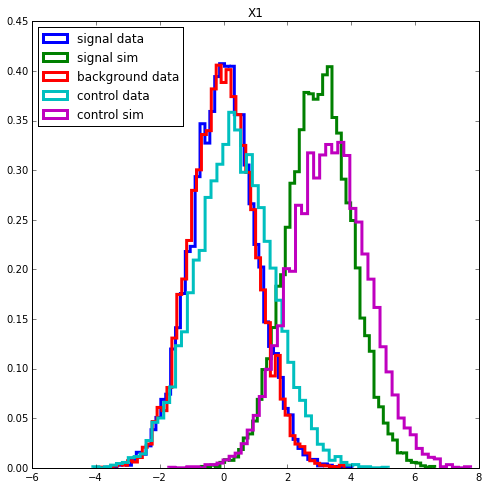
\includegraphics[width=0.6\textwidth]{x1.png}
\end{figure}

$X_1$ is {\color{red} irrelevant} for real data signal versus real data
background, but relevant for simulated versus real data events.

\end{frame}

\begin{frame}

\begin{figure}
\centering
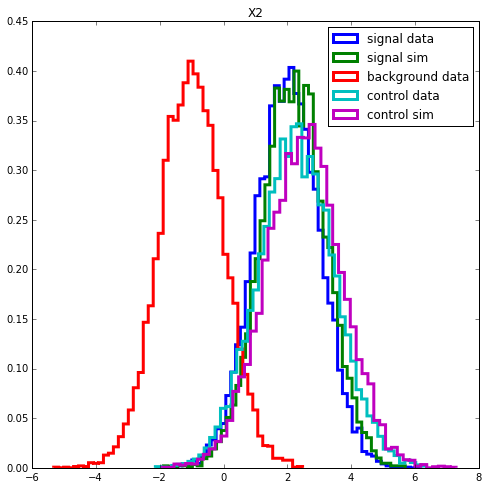
\includegraphics[width=0.6\textwidth]{x2.png}
\end{figure}

$X_2$ is {\color{blue} relevant} for  background and non-background events.

\end{frame}

\begin{frame}

\begin{figure}
\centering
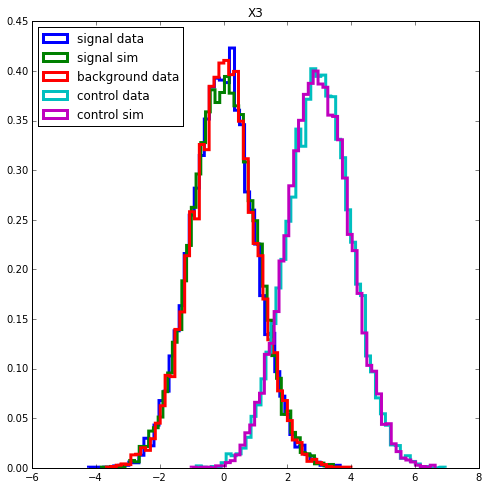
\includegraphics[width=0.6\textwidth]{x3.png}
\end{figure}

$X_3$ is relevant for training versus control events,
but has otherwise no discriminative power between signal and
background events.

\end{frame}

\begin{frame}[fragile]
  \frametitle{Random exploration}

{\scriptsize
\begin{pythoncode}
from sklearn.ensemble import ExtraTreesClassifier

def find_best_tree(X_train, y_train, X_test, y_test,
                   X_data, y_data, X_control_sim, X_control_data):
    best_auc_test, best_auc_data = 0, 0
    best_ks = 0
    best_tree = None

    for seed in range(2000):
        clf = ExtraTreesClassifier(n_estimators=1, max_features=1,
                                   max_leaf_nodes=5, random_state=seed)
        clf.fit(X_train, y_train)
        auc_test = roc_auc_score(y_test, clf.predict_proba(X_test)[:, 1])
        auc_data = roc_auc_score(y_data, clf.predict_proba(X_data)[:, 1])
        ks = ks_statistic(clf.predict_proba(X_control_sim)[:, 1],
                          clf.predict_proba(X_control_data)[:, 1])

        if auc_test > best_auc_test and ks < 0.09:
            best_auc_test = auc_test
            best_auc_data = auc_data
            best_ks = ks
            best_tree = clf

    return best_auc_test, best_auc_data, best_ks, best_tree
\end{pythoncode}
}

\end{frame}

\begin{frame}[fragile]
  \frametitle{Random exploration}

{\scriptsize
\begin{pythoncode}
auc_test, auc_data, ks, tree = find_best_tree(X_train, y_train,
                                              X_test, y_test,
                                              X_data, y_data,
                                              X_control_sim, X_control_data)

# Estimated AUC (simulated signal vs. data background)
>>> 0.986357983199

# True AUC (data signal vs. data background)
>>> 0.90973817

# KS statistic
>>> 0.0578  # < 0.09
\end{pythoncode}
}

\end{frame}

\begin{frame}
What just happened? By chance, we have found a classifier that
\begin{itemize}
\item has seemingly good test performance;
\item passes the control channel test that we have defined.
\end{itemize}
{\color{blue} This classifier appears to be exactly the one we were seeking}.
\vspace{1cm}

{\color{red}Wrong}. The expected ROC AUC of 0.91 on real data signal and real data
background is significantly lower than our first estimate, suggesting that
there is still something wrong.

\end{frame}

\begin{frame}
\begin{figure}
\centering
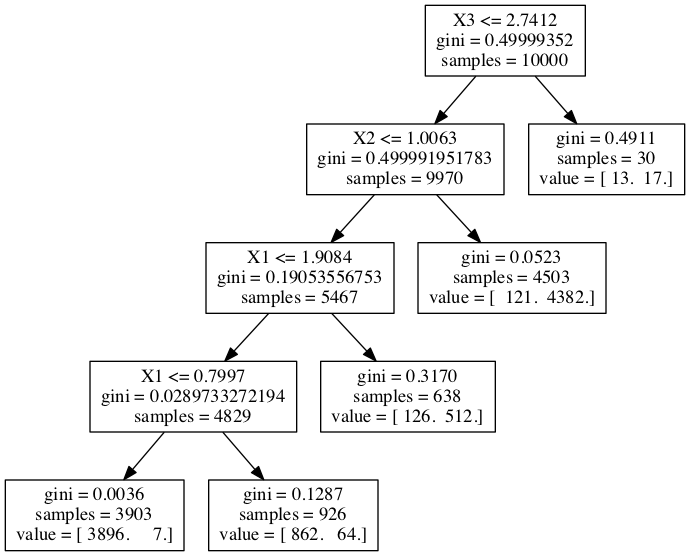
\includegraphics[width=0.7\textwidth]{tree.png}
\end{figure}

$\varphi$ exploits $X_1$, i.e. simulation versus real data
artefacts to indirectly classify signal from background events, {\color{red}while still passing the
control channel test} because of its use of $X_3$!

\end{frame}


\begin{frame}
  \frametitle{Winning the challenge}

% As in the challenge, simulation versus real data patterns may be hidden into
% several variables, making it not possible to detect the problem by eye by
% looking at variables individually. However, a learning algorithm might still be
% able to exploit them, either by chance or on purpose.
%
% \vspace{0.5cm}

\begin{enumerate}
\item learn to distinguish between training and control data,
\item build a classifier on training data, with all the freedom to exploit simulation artefacts,
\item assign random predictions to samples predicted as control data, otherwise predict using the classifier found in the previous step.
\end{enumerate}

\begin{figure}
\centering
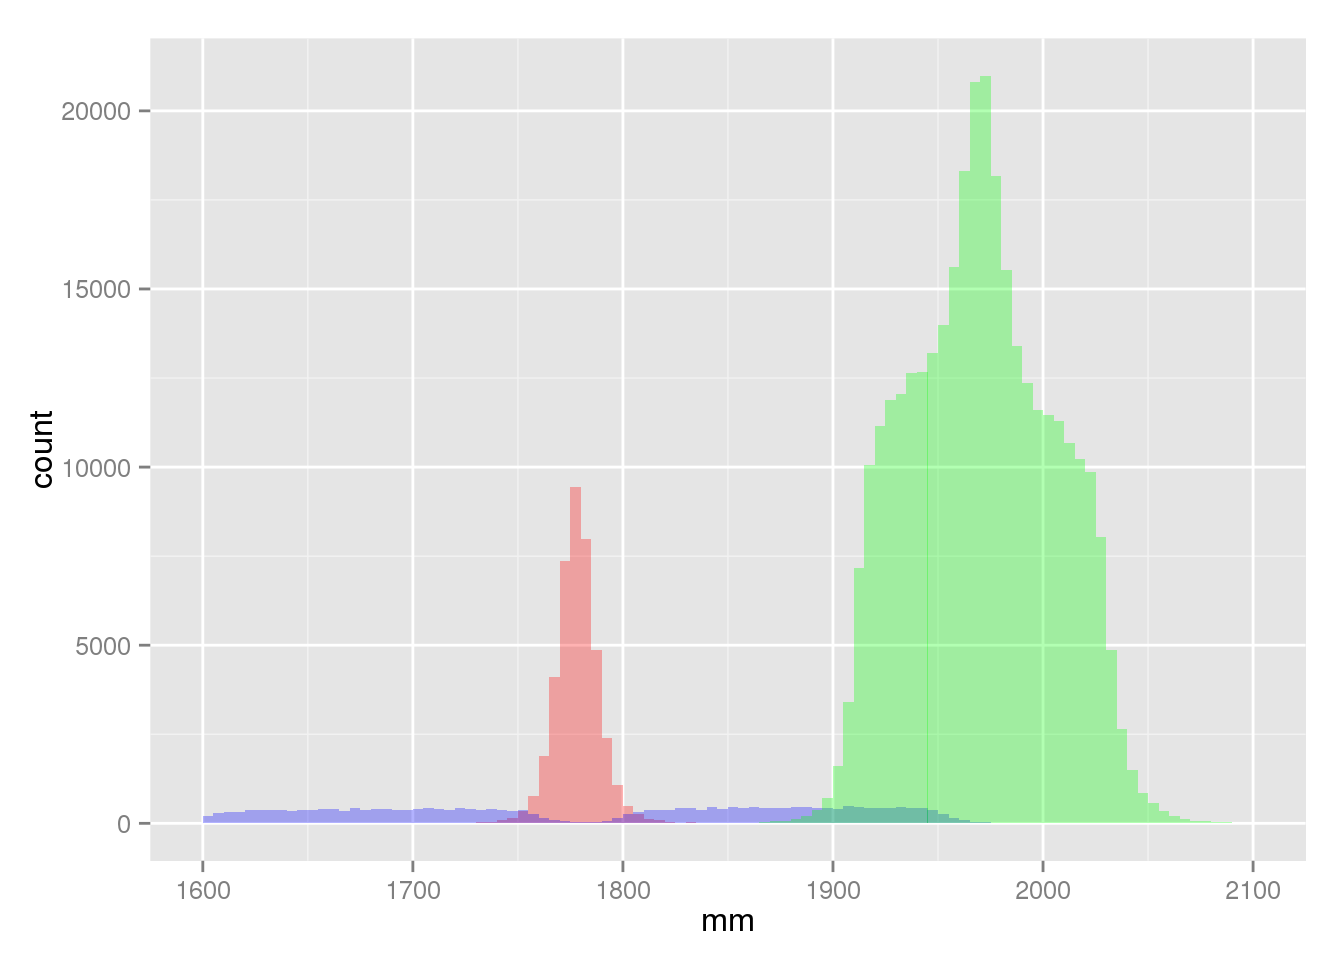
\includegraphics[width=0.5\textwidth]{hole.png}
\end{figure}

\end{frame}

\begin{frame}
  \frametitle{A machine learning response}

\end{frame}

\begin{frame}[t]{Conclusions}
    
\end{frame}
%--- Next Frame ---%

\begin{frame}[t]{References}
    See also our \href{https://github.com/glouppe/notebooks/blob/master/Classification\%20with\%20a\%20control\%20channel.ipynb}{notebook} for further details.
\end{frame}
%--- Next Frame ---%




\end{document}
